\chapter{Artificial Neural Networks}

\section{Theory}
Artificial Neural Networks (ANN) also called multilayer perceptron, can be used as a model for pattern recognition. 
The neural network model is a nonlinear function from a set of input variables $ \left\lbrace x_i \right\rbrace  $ transformed to a set of output variables $ \left\lbrace y_k \right\rbrace  $ controlled by the weight vector \textbf{w}, which is made of adjustable parameters.
The number of hidden units between the input and the output can be adjusted to the dataset, the process is described in the method.

The overall network function for a two layer neural network, takes the form
\begin{equation}
y_k(\mathbf{x},\mathbf{w}) = \sigma \left( \sum_{j=1}^{M} w_{kj}^{(2)} h\left( \sum_{i}^{D} w_{ji}^{(1)} x_i + w_{j0}^{(1)} \right) + w_{k0}^{(2)} \right) 
\label{eq:ANN_overall}
\end{equation}
The superscript (1) and (2) indicates which layer the parameter is in, also shown on the parameters in figure \ref{fig:ANN_fig_theory}. 
Both $ \sigma(\cdot) $ and $ h(\cdot) $ are activation functions, which can be chosen to be either the logistic sigmoid or the tanh function.
The part with $ h(...) $ is in the context of ANN called the hidden units. 
D is the number of inputs, M is the number of hidden units and K is the number of outputs.


  
\begin{figure}[H]
\centering
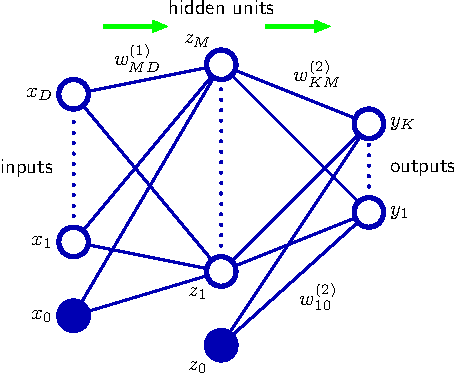
\includegraphics{Figure5_1}
\caption{Diagram of the two layer neural network. The nodes in the figure represents the input, hidden and output variable. The links between the nodes are the weight parameters. The figure is borrowed from \cite{bishop2007}} 
\label{fig:ANN_fig_theory}
\end{figure}

\section{Method}
In both the training and test phases the Netlab Toolbox  was used in MATLAB.
In the training of the neural network for a multi-class classification problem the following error-function is minimized.
\begin{equation}
E(\mathbf{w}) = \dfrac{1}{2} \sum_{n=1}^{N}\| \mathbf{y}(\mathbf{x}_n,\mathbf{w})-\mathbf{t}_n \|^2+\lambda| \mathbf{w}^T \cdot \mathbf{w}|
\label{eq:ANN_error}
\end{equation}
Where $ \mathbf{y}(\mathbf{x}_n,\mathbf{w}) $ is the network function with the parameters and biases in $ \mathbf{w} $ and the target vector, $ \mathbf{t}_n $, is written as a one-of-K-coding.
By minimizing the error-function the parameter that are best for classifying this type of data is fund. 
The parameter include number hidden units and the $\alpha$, which is the inverse variance of the Gaussian noise.
The dataset that was used on the error-function, was the single digit data.
The reason for this, is the vast time it takes to minimizing the error-function, therefore the smallest dataset is used.
This can however make a small error in the number of hidden units optimal for the big dataset of ten digits. 
The number numbers of hidden units found to be optimal is 30, this is used on all of the dataset.

\section{Results}
Using ANN has been tried with different data complexities.
Most notably, with speakers uttering the same single digit ("\textit{ZERO}"), two different digits ("\textit{ZERO}" and "\textit{ONE}"), and ten different digits ("\textit{ZERO}", "\textit{ONE}" through "\textit{NINE}").

\subsection{Single digit:}
\begin{figure}[H]
\centering
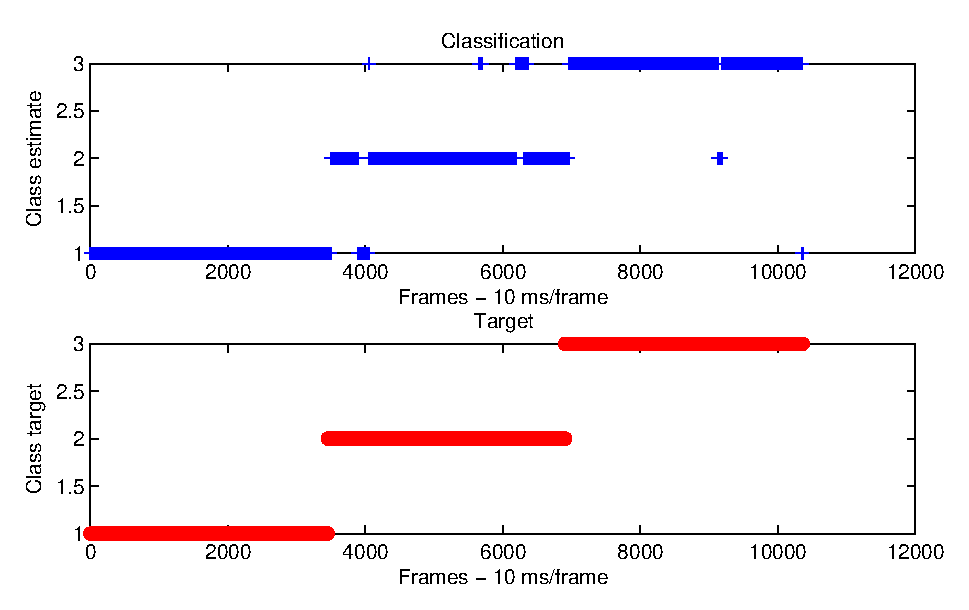
\includegraphics{ANN_1digit_8cent_3speak}
\caption{Results of using ANN with 3 speakers, 30 hidden variables and 1 digit spoken}
\label{fig:ANN_fig_1}
\end{figure}

\begin{table}[H]                                                    
\centering                                                          
\begin{tabular}{|l|c|c|c|c|}                                        
\hline                                                              
  & Speaker Jacob & Speaker Mose & Speaker Simon & Precision [\%] \\
\hline                                                              
Estimate Jacob & 3454.0 & 196.0 & 11.0 & 94.3 \\                    
\hline                                                              
Estimate Mose & 0.0 & 3077.0 & 104.0 & 96.7 \\                      
\hline                                                              
Estimate Simon & 0.0 & 181.0 & 3339.0 & 94.9 \\                     
\hline                                                              
Sensitivity [\%] & 100.0 & 89.1 & 96.7 & 95.3 \\                    
\hline                                                              
\end{tabular}                                                       
\caption{Confusion matrix - 1 digit}                                
\label{table:ANN_conf_1}                                            
\end{table}  



\subsection{Two digits:}
\begin{figure}[H]
\centering
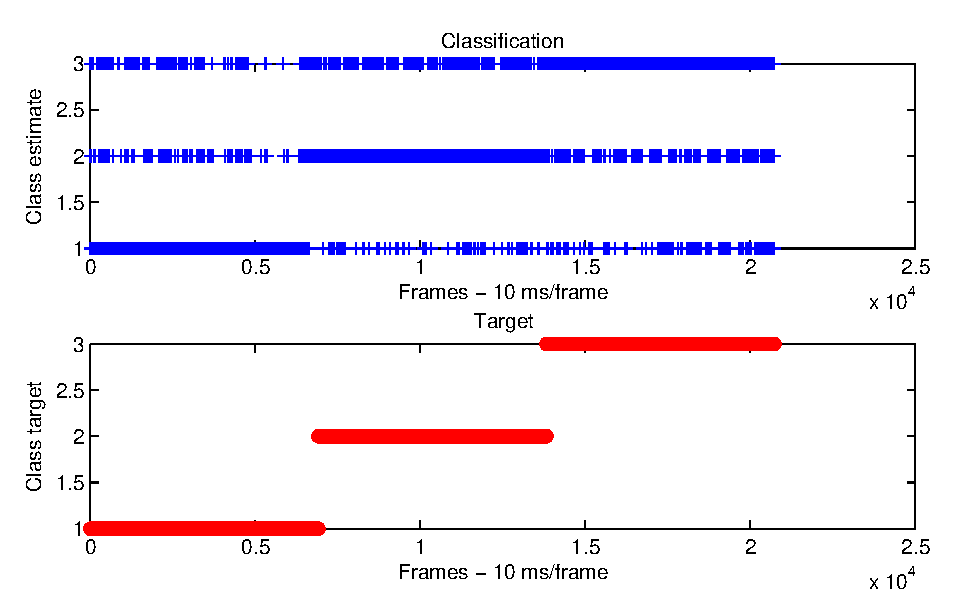
\includegraphics{ANN_2digit_8cent_3speak}
\caption{Results of using ANN with 3 speakers, 30 hidden variables and 2 digits spoken}
\label{fig:ANN_fig_2}
\end{figure}

\begin{table}[H]                                                    
\centering                                                          
\begin{tabular}{|l|c|c|c|c|}                                        
\hline                                                              
  & Speaker Jacob & Speaker Mose & Speaker Simon & Precision [\%] \\
\hline                                                              
Estimate Jacob & 6486.0 & 0.0 & 93.0 & 98.6 \\                      
\hline                                                              
Estimate Mose & 276.0 & 6485.0 & 492.0 & 89.4 \\                    
\hline                                                              
Estimate Simon & 148.0 & 425.0 & 6325.0 & 91.7 \\                   
\hline                                                              
Sensitivity [\%] & 93.9 & 93.8 & 91.5 & 93.1 \\                     
\hline                                                              
\end{tabular}                                                       
\caption{Confusion matrix - 2 digits}                               
\label{table:ANN_conf_2}                                            
\end{table}



\subsection{Ten digits:}
\begin{figure}[H]
\centering
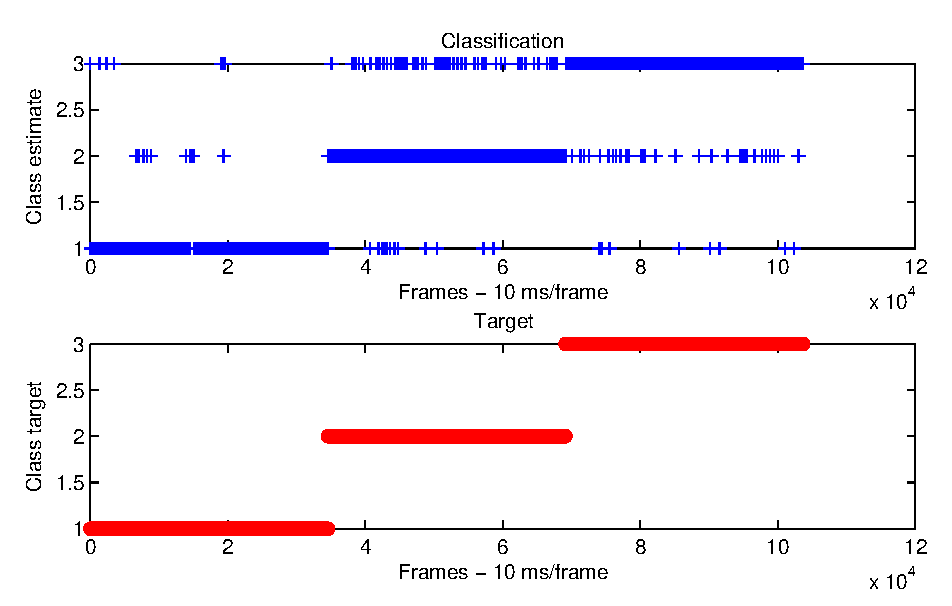
\includegraphics{ANN_10digit_8cent_3speak}
\caption{Results of using ANN with 3 speakers, 30 hidden variables and 10 digits spoken}
\label{fig:ANN_fig_10}
\end{figure}

\begin{table}[H]                                                    
\centering                                                          
\begin{tabular}{|c|c|c|c|c|}                                        
\hline                                                              
  & Speaker Jacob & Speaker Mose & Speaker Simon & Precision [\%] \\
\hline                                                              
Estimate Jacob & 32915.0 & 1186.0 & 528.0 & 95.1 \\                 
\hline                                                              
Estimate Mose & 1245.0 & 28807.0 & 3100.0 & 86.9 \\                 
\hline                                                              
Estimate Simon & 399.0 & 4566.0 & 30931.0 & 86.2 \\                 
\hline                                                              
Sensitivity [\%] & 95.2 & 83.4 & 89.5 & 89.4 \\                     
\hline                                                              
\end{tabular}                                                       
\caption{Confusion matrix - 10 digits}                              
\label{table:ANN_conf_10}                                           
\end{table}


\section{Discussion}
In this project there the three test dataset.
The CM of one digit is displayed on table \ref{table:ANN_conf_1}, The overall accuracy of the linear classification is  calculated to 95.3 \%.
The CM of two digits is displayed on table \ref{table:ANN_conf_2}, The overall accuracy of the linear classification is  calculated to 93.1 \%.
The CM of ten digits is displayed on table \ref{table:ANN_conf_10}, The overall accuracy of the linear classification is  calculated to 89.4 \%.
The CM of the classification show that the model has decreasing accuracy for higher numbers of digits.
This probably because of the number of hidden units is calculated for the dataset of one digit.
The result could be optimized for larger number of digits, if the minimization of the  error-function was used on the other dataset.
This was not done because the process is very time consuming.
 
The overall accuracy of the ANN model is very good, and the model can be used as an reliable speaker recognition classifier.    
In this project the best model to recognise a speaker is the Artificial Neural Networks, with the highest overall accuracy.  